\documentclass[11pt]{article}

\usepackage[margin=1in]{geometry}
\usepackage{amsmath,amssymb,amsthm,mathtools}
\usepackage{booktabs,array}
\usepackage{graphicx}
\usepackage{float}
\usepackage{microtype}
\usepackage{setspace}
\usepackage{enumitem}
\usepackage[round,authoryear]{natbib}
\usepackage[colorlinks=true,allcolors=blue]{hyperref}

\newtheorem{proposition}{Proposition}
\newtheorem{definition}{Definition}
\newtheorem{assumption}{Assumption}
\newtheorem{remark}{Remark}
\theoremstyle{definition}
\newtheorem{conditionalresult}{Conditional result}

\newcommand{\dd}{\,\mathrm{d}}
\newcommand{\gA}{g_A}
\newcommand{\gY}{g_Y}
\newcommand{\gw}{g_w}
\newcommand{\sX}{s_X}
\newcommand{\sM}{s_M}
\newcolumntype{P}[1]{>{\raggedright\arraybackslash}p{#1}}

\title{The Future of Growth and Human Labor under Automated AI Research:\\
AI Capability as Research-Augmenting Technology}
\author{Oliver Pardo}
\date{August 2026}

\begin{document}
\maketitle

\begin{abstract}
This paper develops an endogenous-growth model in which current AI capability
turns compute into both production services and automated research services. A
monopolist supplies AI services and invests in better AI using human researchers
and research compute. Final output combines capital with a CES aggregate of labor
and AI services. When labor and AI services are complements, labor remains a
long-run bottleneck. At unit elasticity between labor and AI services, balanced
growth requires diminishing returns to research to dominate the feedback from
better AI to production and to AI research itself. When these inputs are
substitutes, an interior path with unbounded AI improvement cannot have finite
constant growth rates. Along a regular AI-dominated limit, growth accelerates
while labor's income share
vanishes, but real wages eventually rise when substitution is below an explicit
threshold. Perfect-foresight simulations illustrate the transition toward the
unit-elasticity balanced-growth limits.
\end{abstract}

\onehalfspacing

\section{Introduction}

The economic question is not only whether artificial intelligence can perform
tasks currently done by workers. It is also whether AI can perform the research
that produces better AI. Once the same technology enters both current production
and the improvement of future technology, a familiar substitution problem becomes
a dynamic feedback problem. Better AI lowers the compute cost of AI services,
raises output and the resources available for research, and makes research compute
itself more productive. Whether that loop settles into balanced growth or instead
accelerates depends on where human labor remains essential.

This paper studies that feedback in a general-equilibrium growth model. Raw
compute has two uses. Inference compute is transformed by current AI capability
into services used in final production. Research compute is transformed by the
same capability into automated research services. Human researchers and automated
research services are combined with a CES technology to improve AI capability.
An integrated monopolist supplies AI services and chooses its research inputs.
Households own capital and the developer, supply labor, and choose consumption.
Population grows exogenously.

The distinction between raw compute and the services produced by compute is
central. A unit of compute is not a unit of intelligence. Current capability
determines what a given unit of hardware, energy, and datacenter time can produce.
We therefore write production services as the product of capability and inference
compute, and automated research services as the product of capability and research
compute. This symmetric treatment corresponds closely to the distinction between
inference and training compute in \citet{korinekmckelvey2026}. It also removes a
potential inconsistency in models that let capability augment compute in final
production but not in AI research.

The model deliberately excludes a separate standing-on-shoulders term from its
baseline research technology. Better AI affects research only by making research
compute more productive. This choice prevents the model from counting the same
technological feedback twice and makes the source of acceleration transparent. A
direct knowledge-spillover term can be added later, but it is not needed for the
mechanism studied here.

The analysis separates three regimes according to the elasticity of substitution
between labor and AI services in final production. When the elasticity is below
one, the monopoly supplies a finite ratio of AI services to labor as capability
becomes abundant. The economy then approaches a production technology in capital
and labor alone, so output per capita cannot grow forever along a conventional
balanced path. At unit elasticity, the paper derives the growth rates and resource
shares of balanced-growth candidates. Automating research tightens the relevant
stability condition because capability now raises both inference services and
automated research services. When the elasticity exceeds one, unbounded capability
raises output relative to capital and hence the return to capital without bound.
A finite-rate steady state is impossible.

For the gross-substitutes regime, the paper goes beyond this nonexistence result.
It characterizes an AI-dominated limiting equilibrium in which output, capital,
consumption, and capability accelerate. The result is conditional on the path
remaining interior and on the monopoly solution satisfying its second-order
condition. Within the parameter region for which that limit is established,
labor's share tends to zero, while the real wage rises below an explicit
substitution threshold and falls above it. This distinction
between labor's share and the wage is economically important: a factor may receive
a vanishing fraction of an economy that is expanding even faster.

Perfect-foresight simulations solve the household Euler equation, the developer's
research first-order conditions and costate equation, the monopoly pricing
condition, both market-clearing conditions, and the two laws of motion. The
simulations are used to illustrate propositions, not to replace them. The reported
paths are rejected unless their resource, optimality, and dynamic residuals are
small.

The paper contributes in three ways. First, it provides a symmetric accounting of
inference and research compute. Second, it shows exactly how this accounting
changes the balanced-growth denominators: capability enters automated research
through the product of capability and research compute. Third, it separates the
long-run behavior of wages from the long-run behavior of labor's income share on
an accelerating equilibrium path. These results connect the literature on
research-based growth, automation, factor substitution, and economic singularities
within one tractable model.

\section{Related literature}

The research technology belongs to the tradition of endogenous and
semi-endogenous growth models in which resources devoted to ideas determine the
evolution of productivity \citep{romer1990,aghionhowitt1992,jones1995}. The
population term matters for the same reason it matters in \citet{jones1995}: when
human researchers remain essential, growth in the research workforce can anchor
long-run innovation. The present model asks when that anchor disappears because
capability-augmented research services can substitute for human researchers. Its
homothetic CES research technology separates the elasticity of
substitution from returns to research scale. This distinction preserves the
diminishing-returns margin in idea production emphasized by \citet{jones1995}
while allowing the model to study whether the input mix becomes increasingly
automated.

The paper is closely related to work on AI and economic growth.
\citet{aghionjonesjones2019} organize the possibility that automation of the idea
production function may generate very rapid growth and use ``singularity'' for a
finite-time divergence. \citet{nordhaus2021} develops empirical diagnostics for
an economic singularity, while \citet{trammellkorinek2023} studies growth under
transformative AI. \citet{jones2025rd} focuses directly on AI in research and
development. Our contribution is narrower but more explicit about equilibrium
prices and factor substitution: the same capability stock augments compute used
for inference and compute used to improve AI.

The terminology used to distinguish inference output, training activity,
algorithms, and model capital is informed by the economic accounting proposed by
\citet{korinekmckelvey2026}. Their framework treats compute as a central input
allocated between inference and training. In our notation, raw inference compute
and raw research compute are paid uses of final output; current AI capability
transforms them into economically useful services. The stock of capability is
closer to an index of model quality and algorithmic efficiency than to a physical
quantity of chips. The flow of capability improvement corresponds to the formation
of better model capital, broadly construed to include training, post-training,
experimentation, and algorithmic advances.

The final-production block connects to the older literature on the elasticity of
substitution and growth \citep{pitchford1960,jonesmanuelli1990,rebelo1991}. CES
production is not a cosmetic generalization of Cobb--Douglas: whether the
elasticity lies below or above one governs whether labor remains a bottleneck or
AI services can asymptotically dominate along the paths studied here. Empirical work such as
\citet{duffypapageorgiou2000} illustrates why the aggregate elasticity should not
be imposed without scrutiny. \citet{aumshin2024} sharpen this point by estimating
complementarity between equipment and labor but gross substitution between
software and labor. Their estimates do not calibrate our AI-service elasticity,
but they support separating software-like inputs from undifferentiated physical
capital.

The wage and factor-share results relate to the task and automation literature.
\citet{acemoglurestrepo2019} emphasize displacement and reinstatement of labor in
a task framework, and \citet{acemoglu2025} studies the macroeconomic gains from AI
through task exposure. That literature distinguishes tasks---units of work used
in production---from jobs, which bundle several tasks. Automation can therefore
change the tasks performed within a job without eliminating the job itself. Our
model abstracts from task content, occupations, and the creation of new human
tasks. Labor is an aggregate input and full employment holds by construction.
The results should therefore be interpreted as model implications for wages,
factor shares, and sectoral labor allocation, not as predictions about the number
of jobs displaced. Within that abstraction, the model shows how a wage can rise
even when labor income as a share of output falls because the scale of output
changes endogenously.
This mechanism is related to the distinction between wages and labor income shares
emphasized by \citet{autorkausik2026}, but here it is generated by AI research
feedback and monopoly supply. \citet{trammellkorinek2023} likewise show that wages
can rise or fall when output expands and labor income as a share of output contracts. Our conditional
AI-dominated limit maps that ambiguity into an explicit threshold for the
elasticity between labor and AI services.

Finally, the integrated developer connects the analysis to the emerging literature
on AI market structure \citep{korinekvipra2025,gans2024,demireretal2025}. Monopoly
and integration enter through separate channels: the developer charges a markup
on production AI services and internalizes the future operating profits created
by better capability. The present paper
holds market structure fixed in order to isolate the technology. Comparing this
benchmark with monopolistic competition is a natural next step.

\section{Model}

Time is continuous. Population grows at rate \(n\), and people work either in
final production or AI research:
\begin{equation}
 \dot N=nN,\qquad N=L+H.
 \label{eq:axm-labor-market}
\end{equation}
Here \(L\) always denotes production labor and \(H\) human research labor.

\subsection{Household and final production}

The representative household maximizes
\[
 \int_0^\infty e^{-\rho t}N_t\log(C_t/N_t)\,\dd t
\]
and owns physical capital and the AI developer. Its interior Euler equation in
aggregate variables is
\begin{equation}
 \frac{\dot C}{C}=n+\alpha\frac{Y}{K}-\delta-\rho.
 \label{eq:axm-euler}
\end{equation}
Competitive final-good firms produce
\begin{align}
 Y&=K^\alpha Z^{1-\alpha},\\
 Z&=\left[\omega_L L^{\frac{\sigma_{XL}-1}{\sigma_{XL}}}
 +\omega_X X^{\frac{\sigma_{XL}-1}{\sigma_{XL}}}\right]^{
 \frac{\sigma_{XL}}{\sigma_{XL}-1}},
 \qquad \omega_L+\omega_X=1.
 \label{eq:axm-final-production}
\end{align}
The Cobb--Douglas limit is \(Z=L^{\omega_L}X^{\omega_X}\). Define the CES
contribution share of AI services as
\begin{equation}
 s_X=\frac{\omega_X X^{(\sigma_{XL}-1)/\sigma_{XL}}}
 {\omega_L L^{(\sigma_{XL}-1)/\sigma_{XL}}
 +\omega_X X^{(\sigma_{XL}-1)/\sigma_{XL}}}.
 \label{eq:axm-sx}
\end{equation}
Factor prices then satisfy
\begin{equation}
 w=(1-\alpha)(1-s_X)\frac{Y}{L},\qquad
 p_X=(1-\alpha)s_X\frac{Y}{X}.
 \label{eq:axm-factor-prices}
\end{equation}

\Needspace{11\baselineskip}
\begin{remark}[Tasks, jobs, and labor services]
The inputs \(L\) and \(H\) are quantities of homogeneous labor services, not
numbers of tasks, occupations, or jobs. A job can combine several tasks, and AI
can replace some of them without eliminating the job. The model abstracts from
that margin. In addition, \(N=L+H\) imposes full employment: people can move
between final production and AI research, but the model contains neither
unemployment nor job creation and destruction. Consequently, \(\sigma_{XL}\)
measures substitution between aggregate labor and AI services in final
production. It is not a task-level elasticity or a direct measure of the number
of jobs displaced by AI. The model's labor-market predictions concern wages,
factor shares, and the allocation of labor between the two sectors.
\end{remark}

\subsection{Two uses of compute}

\(A\) indexes current AI capability: what one unit of compute can accomplish.
\(U\) is inference compute and \(M\) is research compute. Their service flows are
\begin{equation}
 X=AU,\qquad R=AM.
 \label{eq:axm-two-compute-services}
\end{equation}
\(R\) is only shorthand for automated research services. The paid inputs are
\(U\) and \(M\). Because both uses have the same constant unit cost, we choose
units of raw compute so that one unit costs one unit of final output. This is a
normalization, not an assumption that compute is economically free. To see this,
start from a common cost \(\xi>0\), define
\(\widetilde U=\xi U\), \(\widetilde M=\xi M\),
\(\widetilde A=A/\xi\), \(\widetilde\chi=\chi/\xi\), and, for the shadow
value used below, \(\widetilde q=\xi q\), and then drop tildes.
Both service flows and all resource costs are unchanged. A unit of either AI
service therefore has marginal cost \(1/A\). This separates the capability stock
\(A\), two raw compute inputs \(U,M\), and the two service flows \(X,AM\).

\subsection{AI research}

Human researchers and automated research services produce effective research:
\begin{align}
 E&=\left[\omega_H H^{\frac{\sigma_{HM}-1}{\sigma_{HM}}}
 +\omega_M(AM)^{\frac{\sigma_{HM}-1}{\sigma_{HM}}}\right]^{
 \frac{\sigma_{HM}}{\sigma_{HM}-1}},
 \qquad \omega_H+\omega_M=1,\\
 \dot A&=\chi E^\eta,\qquad 0<\eta<1.
 \label{eq:axm-capability-law}
\end{align}
The baseline contains no additional \(A^\phi\) term. Better capability affects
research only by raising the services produced by \(M\). This isolates research
automation and avoids counting the capability feedback twice.

The unit cost of effective research is
\begin{equation}
 P_E=\left[\omega_H^{\sigma_{HM}}w^{1-\sigma_{HM}}
 +\omega_M^{\sigma_{HM}}\left(\frac{1}{A}\right)^{1-\sigma_{HM}}
 \right]^{1/(1-\sigma_{HM})}.
 \label{eq:axm-research-price}
\end{equation}
Conditional input demands are
\begin{equation}
 H=\omega_H^{\sigma_{HM}}\left(\frac{P_E}{w}\right)^{\sigma_{HM}}E,
 \quad
 AM=\omega_M^{\sigma_{HM}}
 \left(AP_E\right)^{\sigma_{HM}}E.
 \label{eq:axm-research-demands}
\end{equation}
The automated contribution share is
\begin{equation}
 s_M=\frac{M}{wH+M}.
 \label{eq:axm-sm}
\end{equation}
By constant returns in \(E\), it is also the elasticity of \(E\) with respect
to \(AM\).

\subsection{Integrated AI developer}

The developer supplies \(X\), pays \(X/A\) for inference compute, hires
\(H\), uses \(M\), and owns \(A\). The inverse elasticity of demand for \(X\) is
\begin{equation}
 \varepsilon_X^{-1}=\frac{1-s_X}{\sigma_{XL}}+\alpha s_X.
 \label{eq:axm-inverse-elasticity}
\end{equation}
On an interior monopoly branch,
\begin{equation}
 p_X(1-\varepsilon_X^{-1})=\frac{1}{A}.
 \label{eq:axm-monopoly-foc}
\end{equation}
Let \(q\) be the current-value shadow price of capability. Research optimality is
\begin{equation}
 q\frac{\partial\dot A}{\partial H}=w,\qquad
 q\frac{\partial\dot A}{\partial M}=1,
 \label{eq:axm-research-focs}
\end{equation}
or, after minimizing the cost of \(E\),
\begin{equation}
 q\chi\eta E^{\eta-1}=P_E.
 \label{eq:axm-research-scale-foc}
\end{equation}
The envelope derivative of operating profit is \(\pi_A=X/A^2\). Moreover,
\(\partial\dot A/\partial A=\eta s_M\dot A/A\) because a fixed \(M\) supplies
more research services when \(A\) rises. The costate equation is
\begin{equation}
 \frac{\dot q}{q}=\alpha\frac{Y}{K}-\delta-\frac{X}{qA^2}
 -\eta s_M\frac{\dot A}{A}.
 \label{eq:axm-costate}
\end{equation}
The last term is the main dynamic difference from research that combines \(H\)
directly with \(M\).

\subsection{Resources and equilibrium}

The resource constraint is
\begin{equation}
 C+\dot K+\delta K+U+M=Y.
 \label{eq:axm-resource}
\end{equation}

\begin{definition}[Equilibrium]
Given \(K(0),A(0),N(0)>0\), an equilibrium consists of paths satisfying household
optimality, competitive final-good demands, the monopoly and research first-order
conditions, the developer's costate and transversality conditions, both
technologies, and the labor and goods market-clearing conditions.
\end{definition}

The system used for computation is explicit. Given \(K,A,N,q\), equations
\eqref{eq:axm-labor-market} and
\eqref{eq:axm-final-production}--\eqref{eq:axm-research-scale-foc} determine the
static allocation. The dynamics are
\begin{align}
 \frac{\dot K}{K}&=\frac{Y-C-U-M}{K}-\delta,\\
 \frac{\dot A}{A}&=\frac{\chi E^\eta}{A},\\
 \frac{\dot C}{C}&=n+\alpha\frac{Y}{K}-\delta-\rho,\\
 \frac{\dot q}{q}&=\alpha\frac{Y}{K}-\delta-\frac{X}{qA^2}
 -\eta s_M\frac{\dot A}{A}.
 \label{eq:axm-canonical-system}
\end{align}
\(K\) and \(A\) are predetermined; \(C\) and \(q\) jump to the equilibrium saddle
path. The block is closed by initial \(K,A,N\), the labor and goods market
identities, and the no-Ponzi and transversality conditions. In current-value
notation, the relevant terminal restrictions include
\begin{equation}
 \lim_{t\to\infty}e^{-\rho t}\frac{N_tK_t}{C_t}=0,\qquad
 \lim_{t\to\infty}
 \exp\left\{-\int_0^t\left(\alpha\frac{Y_s}{K_s}-\delta\right)\dd s\right\}
 q_tA_t=0.
 \label{eq:axm-tvc}
\end{equation}
The numerical boundary conditions select the stable path approaching the
analytically characterized limit and are checked against these restrictions.

\begin{definition}[Balanced growth and singularity]
A balanced-growth path has finite constant growth rates and constant limiting
allocation shares. An accelerating path has an output growth rate that does not
converge to a finite constant. Following \citet{aghionjonesjones2019}, a
finite-time singularity occurs when output becomes unbounded at a finite date.
\end{definition}

\section{Analytical results}

The paper focuses on the six configurations in Table
\ref{tab:axm-regime-map}. This keeps the role of each elasticity separate.
Research complementarity, \(\sigma_{HM}<1\), is left for an extension.

\begin{table}[H]
\centering
\small
\setlength{\tabcolsep}{4pt}
\caption{Analytical map}
\label{tab:axm-regime-map}
\begin{tabular}{P{0.14\textwidth}P{0.235\textwidth}P{0.235\textwidth}P{0.235\textwidth}}
\toprule
Research & \(\sigma_{XL}<1\) & \(\sigma_{XL}=1\) & \(\sigma_{XL}>1\)\\
\midrule
\(\sigma_{HM}=1\) &
Labor bottleneck on a regular unbounded-\(A\) limit &
Candidate BGP governed by \(D(\omega_M)\) &
No finite-rate path with unbounded \(A\); the singular form is not characterized\\
\(\sigma_{HM}>1\) &
Same production bottleneck; \(s_M\to1\) if \(Aw\to\infty\) &
Automated candidate BGP governed by \(D(1)\) &
No finite-rate path with unbounded \(A\); conditional singular ratios are characterized\\
\bottomrule
\end{tabular}
\end{table}

\subsection{The price of research automation}

The research block can be understood before solving the dynamics. Dividing the
two conditional demands in \eqref{eq:axm-research-demands} gives
\begin{equation}
 \frac{AM}{H}
 =\left(\frac{\omega_M}{\omega_H}\right)^{\sigma_{HM}}
  (Aw)^{\sigma_{HM}},
 \label{eq:axm-input-ratio}
\end{equation}
and therefore
\begin{equation}
 \frac{s_M}{1-s_M}
 =\left(\frac{\omega_M}{\omega_H}\right)^{\sigma_{HM}}
  (Aw)^{\sigma_{HM}-1}.
 \label{eq:axm-automation-odds}
\end{equation}
The relevant relative price is \(Aw\): the wage relative to the normalized cost
of one unit of automated research services.

\begin{proposition}[Research automation]
\label{prop:axm-research-automation}
Along any interior path on which \(Aw\to\infty\), the automated contribution
to research satisfies
\[
 s_M\to
 \begin{cases}
  0,&\sigma_{HM}<1,\\
  \omega_M,&\sigma_{HM}=1,\\
  1,&\sigma_{HM}>1.
 \end{cases}
\]
For \(\sigma_{HM}>1\), automated research services asymptotically dominate the
research CES even though human research can remain positive at every finite date.
\end{proposition}

The proposition concerns the service \(AM\), not raw compute \(M\). This
distinction is important. A rising \(AM/H\) can reflect more research compute,
better capability, or both.

\subsection{Complementarity in final production}

When \(\sigma_{XL}<1\), the integrated monopolist does not supply an unlimited
ratio \(X/L\) as marginal cost tends to zero. On the regular interior branch, the
zero-marginal-cost limit of \eqref{eq:axm-monopoly-foc} sets marginal revenue to
zero. Hence
\begin{equation}
 s_X\longrightarrow
 \bar s_X=\frac{1-\sigma_{XL}}{1-\alpha\sigma_{XL}}\in(0,1).
 \label{eq:axm-complement-share}
\end{equation}
A constant CES share implies a finite constant \(X/L\).

\begin{proposition}[Labor bottleneck]
\label{prop:axm-complements}
Suppose \(\sigma_{XL}<1\), \(A\to\infty\), the monopoly allocation remains on the
regular interior branch,
\[
 \frac{1}{A(K/L)^\alpha}\to0,
\]
and the economy converges to a finite-rate balanced path. Then \(X/L\) converges
to a finite constant and final production becomes
asymptotically proportional to \(K^\alpha L^{1-\alpha}\). Consequently,
\[
 g_Y=g_K=g_L=n,\qquad g_{Y/N}=0,\qquad g_w=0.
\]
\end{proposition}

This is a conditional long-run result, not an existence theorem. In particular,
the declining marginal value of capability may lead the developer to a research
corner before \(A\) becomes unbounded. What the proposition establishes is that
unbounded AI capability does not by itself sustain per-capita growth when labor
and AI services are complements.

\subsection{The Cobb--Douglas final-production benchmark}

Set \(\sigma_{XL}=1\), and define
\begin{equation}
 \beta=(1-\alpha)\omega_X,\qquad
 \lambda=(1-\alpha)\omega_L,\qquad
 \nu=\frac{\beta}{\lambda}=\frac{\omega_X}{\omega_L}.
 \label{eq:axm-cd-definitions}
\end{equation}
The monopoly condition implies
\begin{equation}
 \frac{U}{Y}=\beta^2,
 \label{eq:axm-inference-share-cd}
\end{equation}
and the reduced production equation is
\begin{equation}
 Y^{1-\beta}
 =K^\alpha L^\lambda(\beta^2A)^\beta.
 \label{eq:axm-reduced-cd}
\end{equation}
If \(L\) and \(K,Y\) grow at their balanced rates, this equation gives
\begin{equation}
 g_Y=n+\nu g_A.
 \label{eq:axm-output-growth-cd}
\end{equation}

It is useful to treat Cobb--Douglas research and asymptotically automated research
separately. Let
\begin{equation}
 \bar s=
 \begin{cases}
  \omega_M,&\sigma_{HM}=1,\\
  1,&\sigma_{HM}>1\text{ and }Aw\to\infty.
 \end{cases}
 \label{eq:axm-sbar}
\end{equation}
Define the feedback denominator
\begin{equation}
 D(\bar s)=1-\eta\bar s(1+\nu).
 \label{eq:axm-feedback-denominator}
\end{equation}

\begin{proposition}[Balanced-growth candidates at unit elasticity]
\label{prop:axm-cd-bgp}
Suppose \(\sigma_{XL}=1\), research remains interior, its expenditure share has a
positive limit, and \(L/N\) converges to a positive constant.

\begin{enumerate}[label=(\roman*)]
\item If \(\sigma_{HM}=1\), every balanced-growth equilibrium must have
 \(D(\omega_M)>0\).
\item If \(\sigma_{HM}>1\), \(Aw\to\infty\), and the path converges to an
 asymptotically automated balanced-growth limit, that limit must have \(D(1)>0\).
\end{enumerate}

Whenever the relevant denominator is positive, the candidate growth rates are
\begin{equation}
 g_A=\frac{\eta n}{D(\bar s)},\qquad
 g_Y=g_K=g_C=n+\nu g_A,\qquad
 g_w=\nu g_A.
 \label{eq:axm-cd-growth-rates}
\end{equation}
Let \(\gamma=\nu g_A\). Its candidate output shares are
\begin{align}
 u&\equiv\frac{U}{Y}=\beta^2,\\
 i&\equiv\frac{\dot K+\delta K}{Y}
 =\frac{\alpha(n+\gamma+\delta)}{\rho+\delta+\gamma},\\
 m&\equiv\frac{M}{Y}
 =\frac{\beta^2\eta\bar s\,g_A}
 {\rho-n+(1-\eta\bar s)g_A},\\
 c&\equiv\frac{C}{Y}=1-u-i-m.
 \label{eq:axm-cd-shares}
\end{align}
A feasible interior candidate additionally requires
\[
 \rho>n,\qquad
 \rho-n+(1-\eta\bar s)g_A>0,\qquad c>0,
\]
the monopoly second-order condition, a feasible labor allocation, and the
transversality conditions.
\end{proposition}

The proposition states necessary growth restrictions and lists the remaining
conditions needed for existence; it does not infer existence from \(D>0\) alone.
The intuition for \(D\) is direct. A one-percent increase in \(A\) raises
production and hence research compute through \(\nu\). It also raises the services
produced by every unit of research compute directly. The term \(1+\nu\) combines
these two channels. Only the automated contribution \(\bar s\) transmits them
through the research CES, and \(\eta\) scales their effect on capability
improvement.

Because \(D(1)<D(\omega_M)\), gross substitution in research tightens the
balanced-growth restriction. With the benchmark values used below,
\(D(\omega_M)=0.8031\) and \(D(1)=0.4375\); both are positive. Removing an
additional \(A^\phi\) term is decisive for this conclusion: the baseline does not
add a separate knowledge-spillover channel to the feedback already carried by
\(AM\).

\subsection{Gross substitution in final production}

Let
\begin{equation}
 \theta=\frac{1-\alpha}{\alpha}.
 \label{eq:axm-theta}
\end{equation}
When \(\sigma_{XL}>1\), AI services dominate the final CES as their relative
quantity rises. The monopoly condition then implies
\begin{equation}
 \frac{U}{Y}\to(1-\alpha)^2,\qquad
 \frac{Y}{K}\sim \mathcal D A^\theta
 \label{eq:axm-high-sigma-scaling}
\end{equation}
for a positive constant \(\mathcal D\).

\begin{proposition}[No finite-rate steady state with gross substitution]
\label{prop:axm-no-bgp}
Suppose \(\sigma_{XL}>1\), \(A\to\infty\), and the equilibrium remains on an
interior monopoly branch on which \(s_X\to1\). Then there is no steady state with
finite constant growth rates. In particular, \(Y/K\to\infty\), so the gross return
to capital and household consumption growth become unbounded.
\end{proposition}

The proposition is a nonexistence result. It does not, by itself, prove that every
initial condition reaches a singularity: research can shut down, a constraint can
bind, or a different monopoly branch can intervene. The next result characterizes
the accelerating branch when it exists.

\begin{conditionalresult}[AI-dominated singular limit]
\label{prop:axm-singular-limit}
Assume \(\sigma_{XL}>1\), \(\sigma_{HM}>1\), \(0<\eta<1\), and an
interior equilibrium approaches a finite date at which \(A\to\infty\),
\(s_X\to1\), and \(s_M\to1\). Suppose its consumption, investment, and
research-compute shares, \(g_A/(Y/K)\), and \(qA/K\) converge to positive finite
limits, and \(L/N\) converges to a positive limit. Assume these convergences are
asymptotically regular: the growth rate of each convergent ratio, divided by
\(Y/K\), tends to zero. Write \(z=Y/K\) and
\[
 \Delta=1+\theta-\eta,\qquad
 h=\frac{\eta\alpha}{\Delta}.
\]
Then
\begin{align}
 \frac{g_A}{z}&\to h,&
 \frac{U}{Y}&\to(1-\alpha)^2,\\
 \frac{\dot K+\delta K}{Y}&\to\alpha-\theta h,&
 \frac{M}{Y}&\to\frac{\eta(1-\alpha)^2}{\Delta},\\
 \frac{qA}{K}&\to\frac{(1-\alpha)^2}{\eta\alpha},&
 \frac{C}{Y}&\to
 1-(1-\alpha)^2-\alpha+\theta h
 -\frac{\eta(1-\alpha)^2}{\Delta}.
 \label{eq:axm-singular-ratios}
\end{align}
Moreover,
\begin{equation}
 \dot z\sim\theta h z^2.
 \label{eq:axm-z-law}
\end{equation}
Thus the limiting differential equation reaches \(z=\infty\) in finite time.
Labor's production share tends to zero, while
\begin{equation}
 \frac{g_w}{z}\to
 \frac{\alpha-(\sigma_{XL}-1)h}{\sigma_{XL}}>0
 \label{eq:axm-wage-limit}
\end{equation}
which is positive if and only if
\(\sigma_{XL}<1/(\alpha\eta)\).
\end{conditionalresult}

The result characterizes a postulated asymptotic equilibrium branch; it does not
establish that the branch is reached from arbitrary initial conditions. Within
that branch, the model delivers a sharp separation when
\(1<\sigma_{XL}<1/(\alpha\eta)\): labor's share vanishes, but the wage eventually
rises. Above the threshold, the same conditional scaling implies an eventually
falling wage. This final case should not be interpreted without separately
checking monopoly optimality and convergence to the postulated branch.

\section{Numerical equilibrium paths}

\subsection{Benchmark and method}

The numerical experiments are not a calibration exercise. Parameters with
standard macroeconomic counterparts are held fixed, while the two substitution
elasticities define the cases of interest. Table \ref{tab:axm-parameters} reports
the benchmark.

As in the model, raw compute is measured in resource-expenditure units, so its
common unit cost is one and is not a free parameter.

\begin{table}[H]
\centering
\caption{Benchmark parameters}
\label{tab:axm-parameters}
\begin{tabular}{lcl}
\toprule
Parameter & Value & Interpretation\\
\midrule
\(\alpha\) & 0.33 & Capital elasticity in final output\\
\(n\) & 0.012 & Annual population growth\\
\(\delta\) & 0.05 & Annual depreciation\\
\(\rho\) & 0.04 & Household discount rate\\
\(\omega_X\) & 0.20 & AI weight in the final CES\\
\(\omega_M\) & 0.35 & Automated-service weight in research\\
\(\eta\) & 0.45 & Returns to effective research\\
\(\chi\) & 0.01 & Research-productivity normalization\\
\bottomrule
\end{tabular}
\end{table}

Initial \(A\) and \(N\) are normalized to one. Initial capital is chosen near the
limiting capital-output ratio of the unit-elasticity benchmark. The level of
\(\chi\) and the normalizations affect calendar timing, so the very long horizontal
axis should not be read as a forecast. The economically meaningful objects are
the direction of the transition, the limiting rates and shares, and the
comparison across research technologies.

The solver treats \(K\) and \(A\) as predetermined and chooses initial \(C\) and
\(q\) so that the path approaches the relevant terminal equilibrium. At every
collocation node it solves the monopoly supply condition, labor-market clearing,
the dual research problem, both research first-order conditions, and the four
equations in \eqref{eq:axm-canonical-system}.

\subsection{Unit elasticity in final production}

Figure \ref{fig:axm-research-comparison} compares Cobb--Douglas research
\((\sigma_{HM}=1)\) with gross substitution in research
\((\sigma_{HM}=2)\), holding \(\sigma_{XL}=1\). The analytical limits from
Proposition \ref{prop:axm-cd-bgp} are visible. Under Cobb--Douglas research, the
automated contribution is fixed at \(\omega_M=0.35\), capability growth converges
to 0.67 percent, and output-per-capita growth converges to 0.17 percent. With
gross substitution, the automated contribution approaches one, capability growth
converges to 1.23 percent, and output-per-capita growth approaches 0.31 percent.

\begin{figure}[H]
\centering
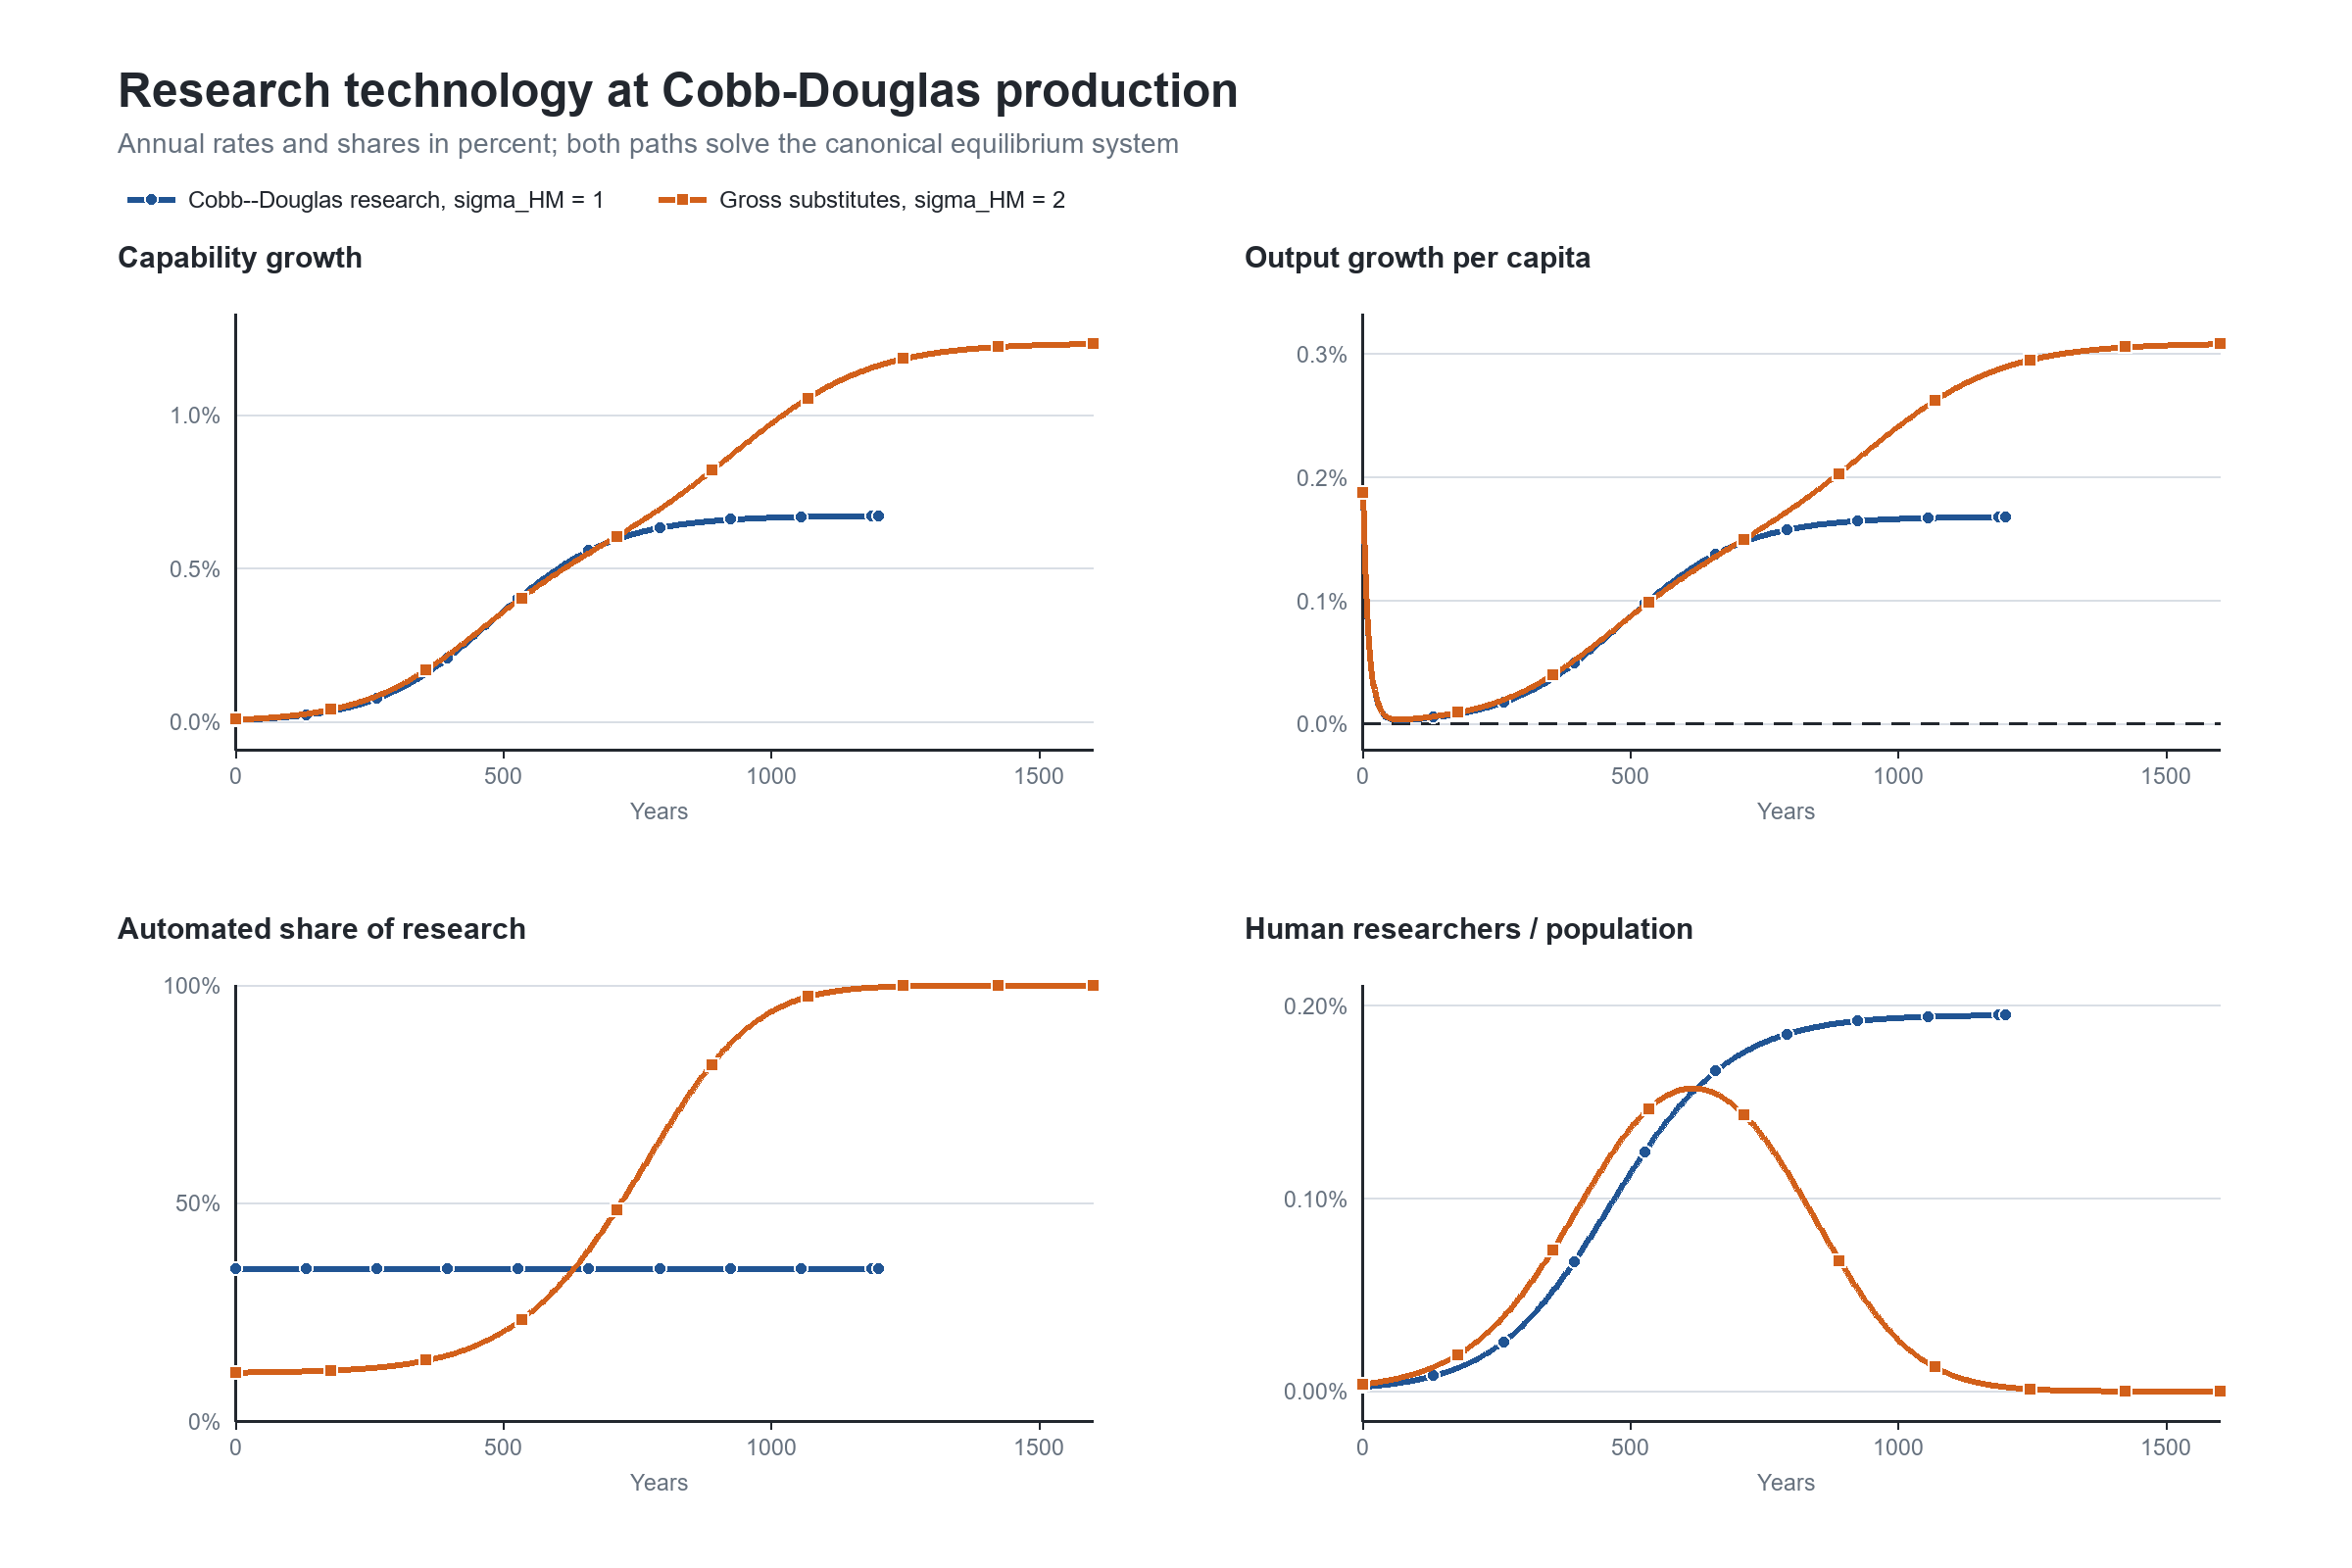
\includegraphics[width=\textwidth]{figures_axm/axm_research_technology_comparison.png}
\caption{Research substitution and the unit-elasticity balanced-growth limit.
Both lines are perfect-foresight equilibrium paths.}
\label{fig:axm-research-comparison}
\end{figure}

The human-research transition contains a result that is hidden by the limiting
research share. With \(\sigma_{HM}=2\), the fraction of the population working in
AI research first rises and later falls toward zero. AI research can therefore
employ more people during the transition even while it becomes progressively more
automated. Under Cobb--Douglas research, the human-research population share
instead converges to a positive constant.

Figure \ref{fig:axm-wages} shows that the distinction between factor prices and
factor shares already matters on these balanced-growth transitions. The real wage
eventually grows at the same rate as output per person, as Proposition
\ref{prop:axm-cd-bgp} requires. The production labor share is fixed by the
Cobb--Douglas final-production technology, while total labor income also includes
human researchers and therefore moves during the research-automation transition.

\begin{figure}[H]
\centering
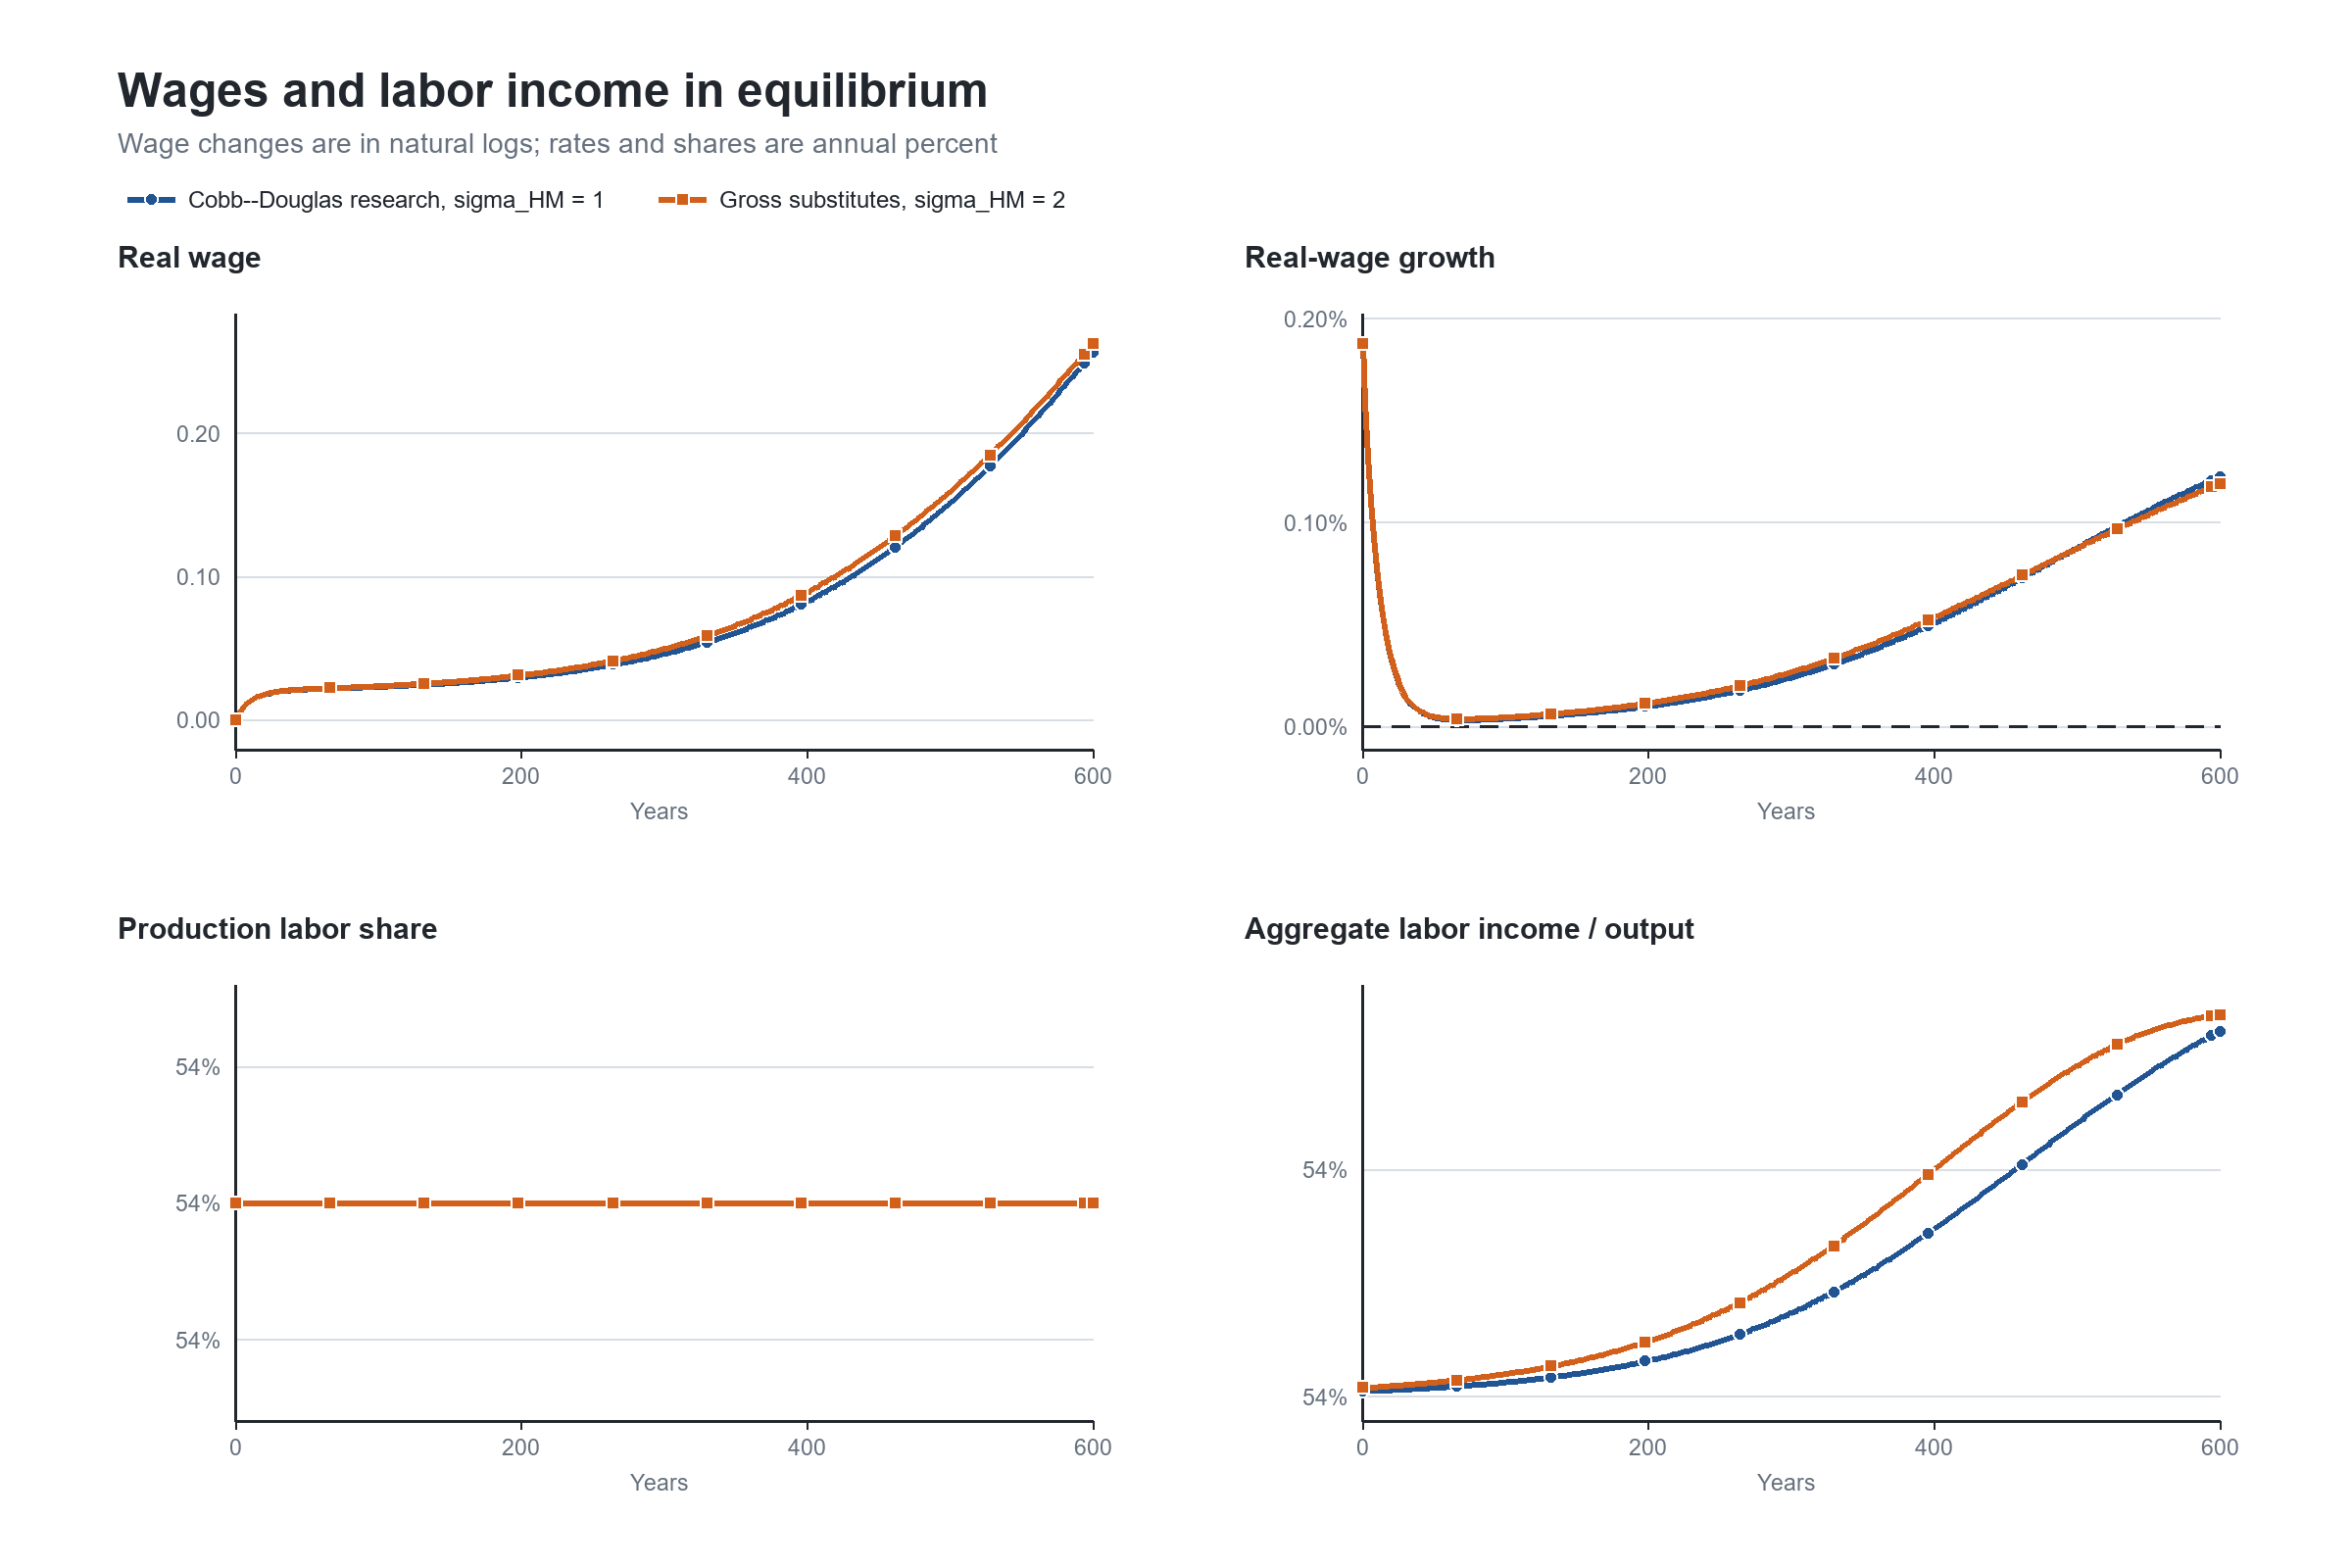
\includegraphics[width=\textwidth]{figures_axm/axm_wages_and_factor_shares.png}
\caption{Real wages and labor income. Both paths satisfy the canonical
equilibrium system.}
\label{fig:axm-wages}
\end{figure}

Figure \ref{fig:axm-research-chain} separates raw research compute \(M\), the
automated services \(AM\), human research \(H\), and effective research \(E\).
This decomposition is essential for interpreting the new specification. Research
compute can grow at one rate while the services produced by that compute grow
faster because capability is improving.

\begin{figure}[H]
\centering
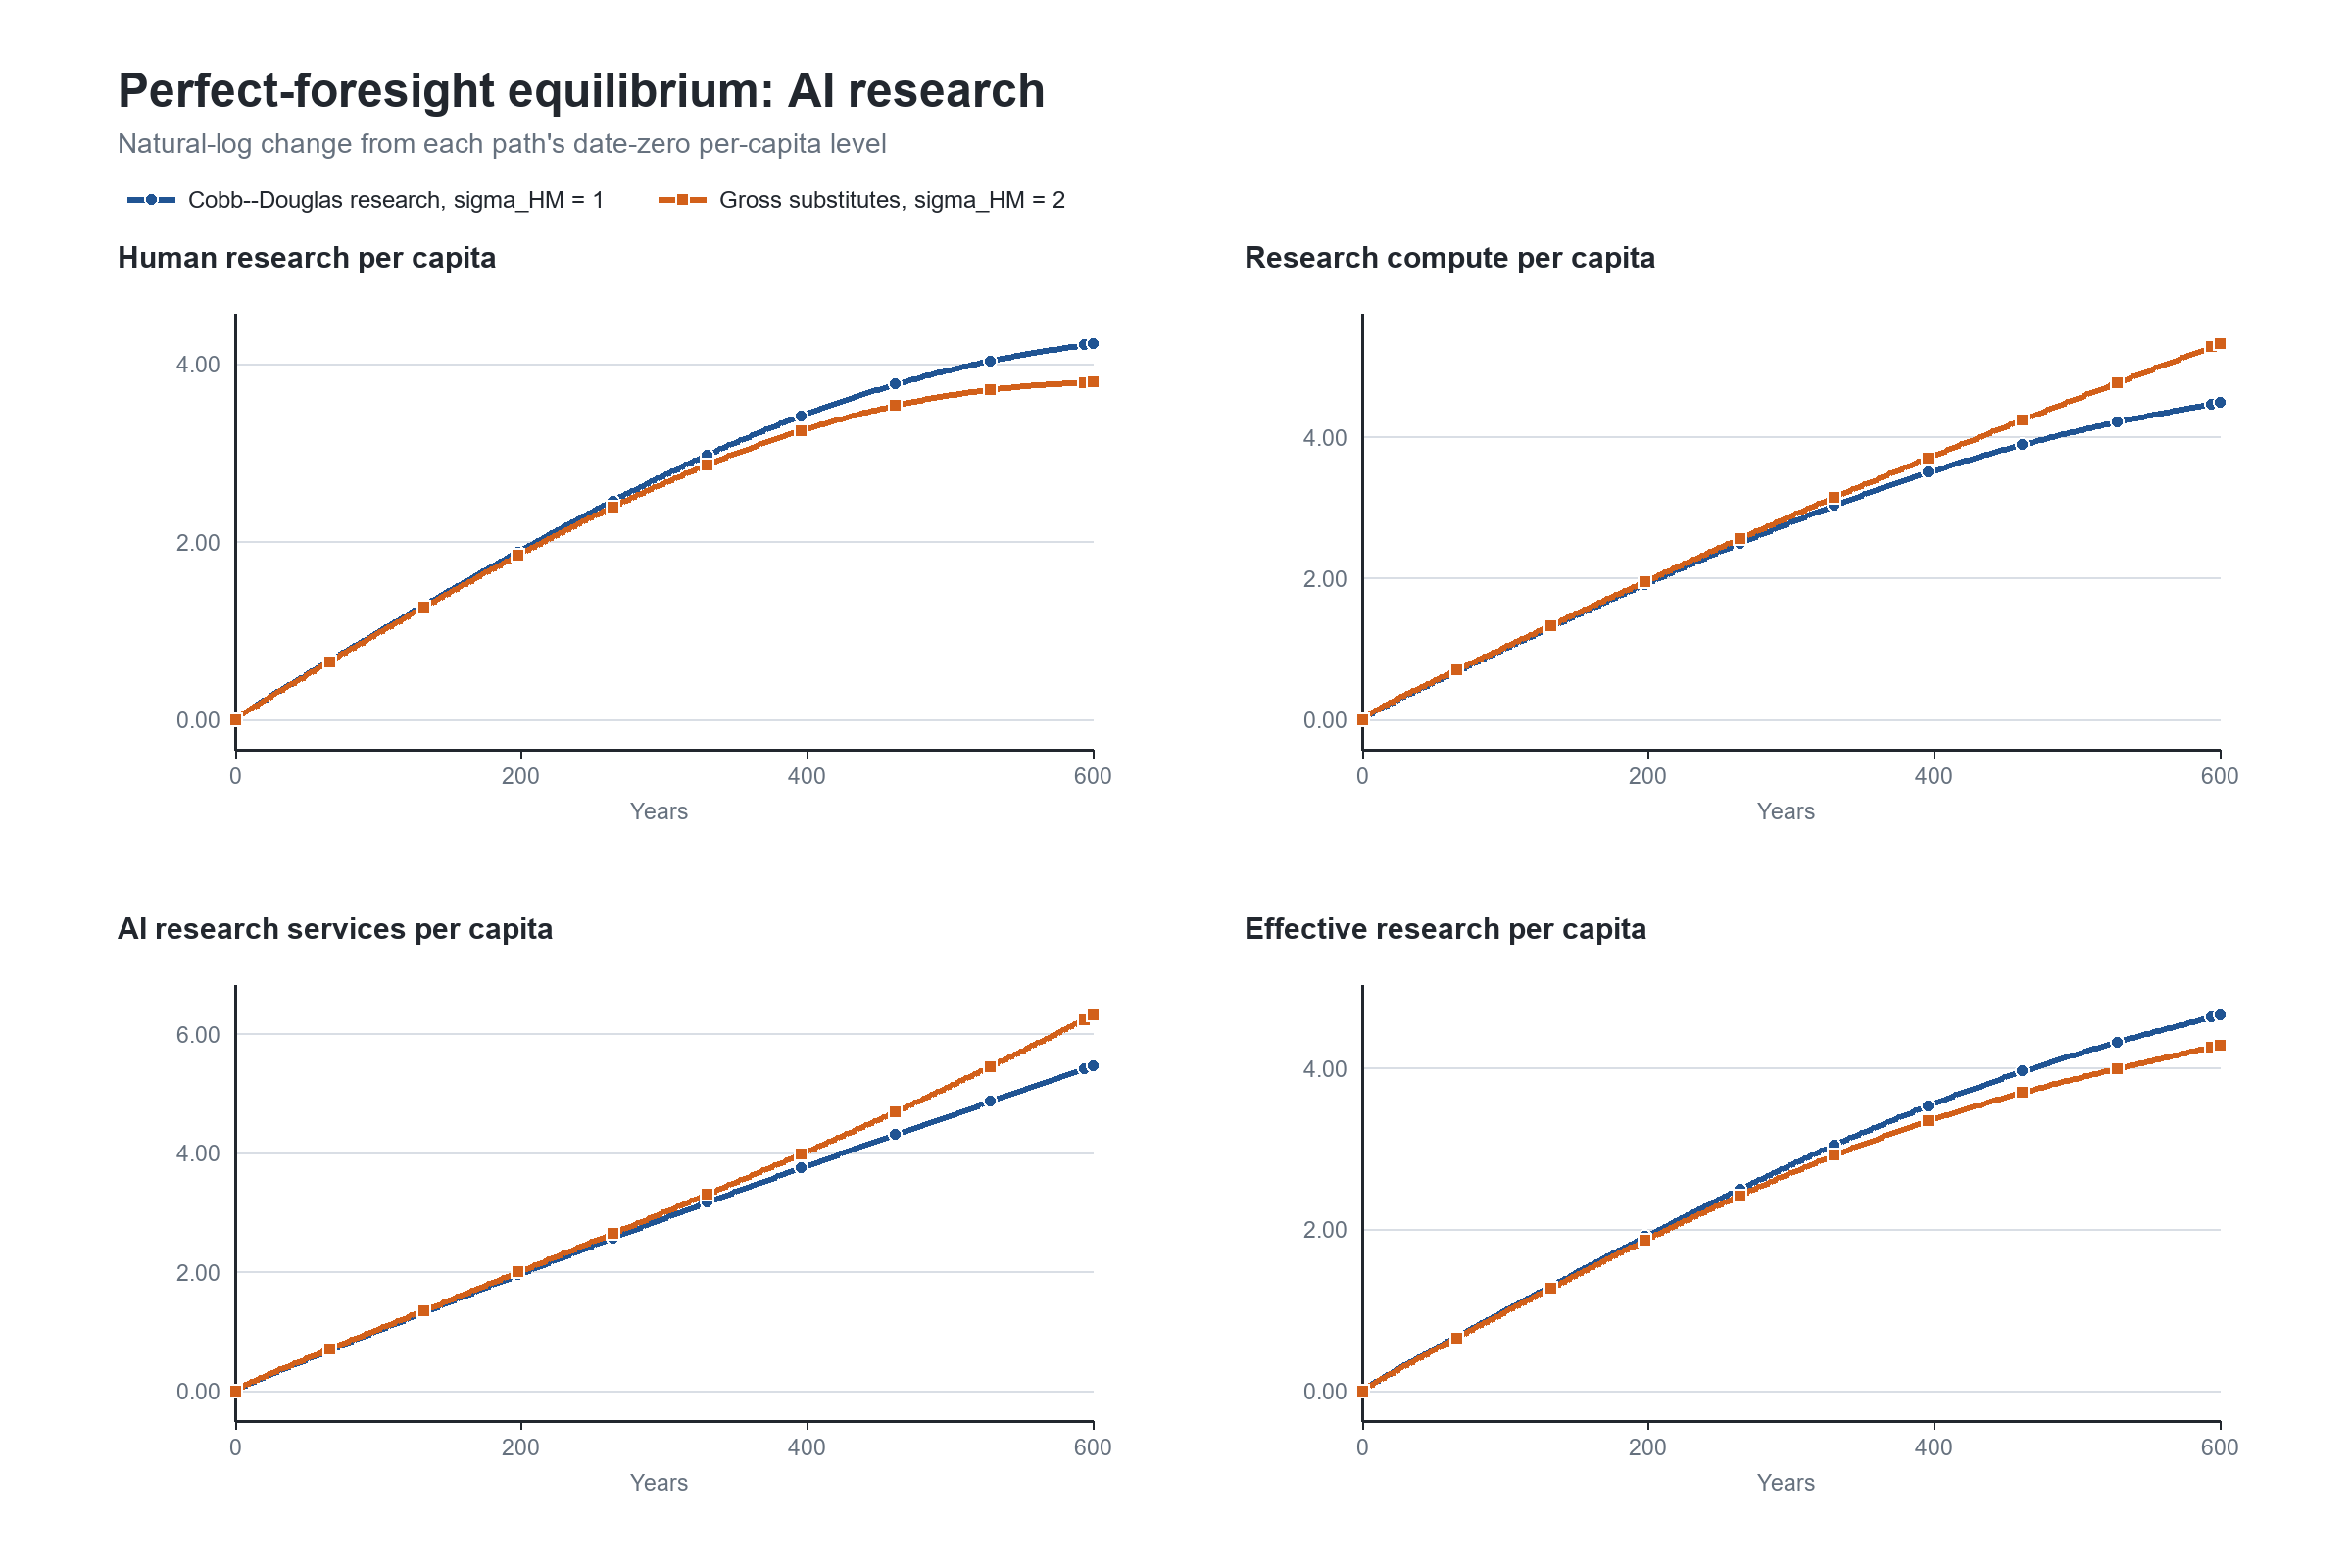
\includegraphics[width=\textwidth]{figures_axm/axm_equilibrium_research_chain.png}
\caption{The AI-research chain. The vertical axes report natural-log changes from
each path's date-zero per-capita level.}
\label{fig:axm-research-chain}
\end{figure}

\subsection{Equilibrium audit}

Table \ref{tab:axm-residuals} reports the numerical audit. The static identities
and first-order conditions are satisfied to approximately machine precision.
The larger numbers are collocation errors in the differential equations and
remain close to \(10^{-5}\). The terminal rates are also close to the analytical
targets despite solving the transition rather than imposing the entire
balanced-growth path.

\begin{table}[H]
\centering
\caption{Equilibrium-path diagnostics}
\label{tab:axm-residuals}
\begin{tabular}{lcc}
\toprule
Diagnostic & \(\sigma_{HM}=1\) & \(\sigma_{HM}=2\)\\
\midrule
Maximum goods-market residual & \(2.2\times10^{-16}\) & \(2.2\times10^{-16}\)\\
Maximum labor-market residual & \(8.9\times10^{-16}\) & \(1.8\times10^{-15}\)\\
Maximum research-FOC log error & \(3.6\times10^{-13}\) & \(1.3\times10^{-11}\)\\
Maximum dynamic path residual & \(4.4\times10^{-6}\) & \(1.2\times10^{-5}\)\\
Terminal automated research share & 0.3500 & 0.99999\\
\bottomrule
\end{tabular}
\end{table}

\subsection{Gross substitution in final production}

For \(\sigma_{XL}>1\), a conventional terminal balanced-growth condition would
contradict Proposition \ref{prop:axm-no-bgp}. We therefore use a separate
free-boundary algorithm that terminates at a large value of \(Y/K\) and imposes
the limiting ratios in Conditional Result \ref{prop:axm-singular-limit}. A path is
reported only after convergence across progressively larger terminal boundaries
and after the same equilibrium-residual audit used above. This prevents a
finite-horizon initial-value path from being mislabeled as an infinite-horizon
equilibrium.

The robust qualitative prediction is analytical: the economy can remain close to
ordinary growth while \(Y/K\) is moderate, but growth and the return to capital
rise together once the AI-dominated scaling becomes quantitatively important. We
do not report a high-substitution curve in the present numerical set. Fixed-horizon
solutions satisfy the local equilibrium equations, but the free-boundary
continuation has not yet passed the convergence test across increasingly distant
terminal boundaries. Presenting such a curve as an equilibrium transition would
therefore overstate what has been verified. The analytical nonexistence and
limiting-ratio results do not depend on that unfinished numerical exercise.

\section{Conclusion}

The paper asks what changes when current AI capability augments not only
inference compute but also compute used to improve AI. The answer is not a
notational detail. It changes the relative price of automated research services,
adds a capability term to the developer's costate equation, and strengthens the
feedback from AI improvement to future AI improvement.

Three results organize the analysis. First, the research elasticity determines
whether a rising wage relative to the price of automated research services makes
automated research asymptotically dominant.
Second, the final-production elasticity determines whether human labor remains a
long-run bottleneck. With complementarity, output per person cannot keep growing
along the balanced path characterized here when production labor remains a
positive population share. At unit
elasticity, a balanced-growth candidate with positive capability growth can be
feasible only when decreasing returns to effective research dominate the
combined effect of capability on inference and automated research. With gross
substitution, if AI services asymptotically dominate final production, unbounded
capability makes \(Y/K\) and the return to capital
unbounded, ruling out finite constant growth rates.

Third, factor shares and factor prices must be distinguished. Along the
AI-dominated accelerating limit, labor's income share tends to zero. Yet the real
wage eventually rises when final-production substitution is below
\(1/(\alpha\eta)\) along the characterized limit; above that threshold the
conditional wage result reverses. A vanishing share does not by itself imply a
falling level when the scale of the economy grows sufficiently fast.
At the threshold itself, the leading asymptotic term is zero and the model does
not sign the eventual wage change.

The perfect-foresight simulations reinforce the analytical results without being
used as proofs. At unit elasticity in final production, both Cobb--Douglas and
gross-substitutes research paths converge to the rates implied by the model.
When automated research services are gross substitutes for human research, the
human-research employment share is hump-shaped: it can increase for centuries in
the numerical normalization before automation eventually dominates. Separating
\(M\) from \(AM\) makes this transition visible. The simulations also confirm
the Euler-equation link between consumption growth and the net real interest
rate. These paths are numerical illustrations, not forecasts of calendar time.

Several extensions are important. A direct standing-on-shoulders term could be
added to determine how much it amplifies the feedback already carried by \(AM\).
Physical capital could enter AI research explicitly, separating chips,
datacenters, energy infrastructure, and model capability. Alternative market
structures could clarify how competition changes the balance between current
inference supply and research investment.

Finally, greater automation of AI research may create agency and supervision
problems that are absent here. If human oversight is needed to keep automated
research aligned with the developer's objective, an integrated monopolist may
internalize part of that problem and moderate research speed. Competing developers
may instead reduce supervision to avoid losing a race. That extension would make
human research valuable not only as a productive input but also as a governance
input. It could provide a disciplined basis for studying subsidies to human AI
research or taxes on insufficiently supervised research automation; those policy
claims require an explicit agency model and do not follow from the present
technology alone.


\appendix
\section{Proofs}

\subsection{Proof of Proposition \ref{prop:axm-research-automation}}

The ratio of the conditional demands in \eqref{eq:axm-research-demands} is
\[
 \frac{AM}{H}
 =\left(\frac{\omega_M}{\omega_H}\right)^{\sigma_{HM}}
  (Aw)^{\sigma_{HM}}.
\]
Because \(s_M/(1-s_M)=M/(wH)=(AM/H)/(Aw)\), substitution yields
\[
 \frac{s_M}{1-s_M}
 =\left(\frac{\omega_M}{\omega_H}\right)^{\sigma_{HM}}
  (Aw)^{\sigma_{HM}-1}.
\]
Taking the stated limit proves all three cases. \(\square\)

\subsection{Proof of Proposition \ref{prop:axm-complements}}

Normalize the monopoly condition by \((K/L)^\alpha\) and write \(x=X/L\).
The normalized marginal cost tends to zero by hypothesis. At an interior
monopoly allocation,
\[
 p_X\left[1-\frac{1-s_X}{\sigma_{XL}}-\alpha s_X\right]=\frac{1}{A}.
\]
On the regular branch, the zero-marginal-cost limit sets the term in square
brackets to zero. Solving gives
\[
 \bar s_X=\frac{1-\sigma_{XL}}{1-\alpha\sigma_{XL}}.
\]
For \(\sigma_{XL}<1\), this number is strictly between zero and one. The CES share
mapping \eqref{eq:axm-sx} is one-to-one in \(X/L\), so \(X/L\) converges to a
finite positive constant. Hence \(Z/L\) converges to a constant and
\(Y\) is asymptotically a constant multiple of \(K^\alpha L^{1-\alpha}\).

Now suppose, as in the proposition, that a finite-rate balanced path exists.
The household Euler equation requires a constant \(Y/K\), while constant
production shares require \(K/L\) to be constant. Since \(L\) grows at \(n\),
\(K,Y\), and \(C\) grow at \(n\). Output per person and the wage are therefore
constant. \(\square\)

\subsection{Proof of Proposition \ref{prop:axm-cd-bgp}}

With \(\sigma_{XL}=1\), the final technology is
\[
 Y=K^\alpha L^\lambda X^\beta.
\]
The inverse demand elasticity is \(1-\beta\), so the monopoly first-order
condition becomes \(\beta p_X=1/A\). Since \(p_XX=\beta Y\),
\(X/A=\beta^2Y\), proving \eqref{eq:axm-inference-share-cd}. Replacing
\(X\) by \(\beta^2AY\) gives \eqref{eq:axm-reduced-cd}. Taking growth rates
and using \(g_K=g_Y\) and \(g_L=n\) yields
\[
 g_Y=n+\nu g_A.
\]

On a balanced path, raw research compute has a constant output share, so
\(g_M=g_Y=n+\nu g_A\). If \(\sigma_{HM}=1\), human research grows at \(n\) and
\[
 g_E=\omega_H n+\omega_M(g_A+g_M)
 =n+\omega_M(1+\nu)g_A.
\]
If \(\sigma_{HM}>1\) and \(s_M\to1\), then \(E\) is asymptotically proportional
to \(AM\), giving
\[
 g_E=g_A+g_M=n+(1+\nu)g_A.
\]
Both cases are \(g_E=n+\bar s(1+\nu)g_A\). Since
\(\dot A=\chi E^\eta\) and a constant \(g_A>0\) requires
\(g_{\dot A}=g_A\),
\[
 g_A=\eta[n+\bar s(1+\nu)g_A].
\]
Solving gives \eqref{eq:axm-cd-growth-rates}; a positive solution requires
\(D(\bar s)>0\).

The Euler equation gives \(K/Y=\alpha/(\rho+\delta+\gamma)\), which implies the
investment share in \eqref{eq:axm-cd-shares}. Let \(m=M/Y\) and
\(u=\beta^2\). The research-compute first-order condition can be written
\[
 q\,\eta\bar s\,\frac{\dot A}{M}=1,
 \qquad\text{so}\qquad
 \frac{qA}{Y}=\frac{m}{\eta\bar s g_A}.
\]
Because this ratio is constant, \(g_q=g_Y-g_A\). The envelope derivative of
operating profits implies
\[
 \frac{\pi_A}{q}
 =\frac{uY/A}{q}
 =\frac{u\eta\bar s g_A}{m}.
\]
Substitute these expressions into the costate equation and use
\(g_Y=n+\gamma\) and the Euler condition:
\[
 n+\gamma-g_A
 =\rho+\gamma-\eta\bar s g_A
  -\frac{u\eta\bar s g_A}{m}.
\]
Solving for \(m\) gives \eqref{eq:axm-cd-shares}. The resource constraint gives
\(c=1-u-i-m\). Positivity, interiority, second-order, and transversality
conditions are separate requirements, as stated. \(\square\)

\subsection{Proof of Proposition \ref{prop:axm-no-bgp}}

Suppose for contradiction that an equilibrium satisfying the hypotheses has
finite constant growth rates. With \(\sigma_{XL}>1\), AI services dominate the
CES as their relative quantity becomes large. The limiting final technology is
proportional to \(K^\alpha X^{1-\alpha}\). The inverse demand elasticity tends
to \(\alpha\), and the monopoly first-order condition implies
\[
 \frac{X}{A}=(1-\alpha)^2Y[1+o(1)].
\]
Substituting \(X\) back into final production gives
\[
 \frac{Y}{K}=\mathcal D A^{(1-\alpha)/\alpha}[1+o(1)]
\]
for \(\mathcal D>0\). Since \(A\to\infty\), \(Y/K\to\infty\). The gross return
to capital \(\alpha Y/K\) therefore diverges. Equation \eqref{eq:axm-euler}
then makes consumption growth unbounded, contradicting finite constant growth.
\(\square\)

\subsection{Derivation of the AI-dominated singular limit}

Let \(z=Y/K\), \(u=U/Y\), \(m=M/Y\), \(i=(\dot K+\delta K)/Y\), and
suppose the limiting shares are positive and constant. Final-production and
monopoly optimality give
\[
 u\to(1-\alpha)^2,\qquad z\sim\mathcal D A^\theta,\qquad
 \theta=\frac{1-\alpha}{\alpha}.
\]
Write \(g_A\sim hz\). The Euler equation and a constant consumption share imply
\[
 \frac{g_Y}{z}\to\alpha.
\]
Since \(g_Y=g_K+g_z\), \(g_K/z\to i\), and \(g_z=\theta g_A\),
\begin{equation}
 i+\theta h=\alpha.
 \label{eq:axm-app-resource-growth}
\end{equation}

Automated research implies \(\dot A\sim\chi(AM)^\eta\). Log-differentiating
\(g_A=\dot A/A\), using \(g_M=g_Y\) for constant \(m\), gives
\[
 g_{g_A}=(\eta-1)g_A+\eta g_Y.
\]
But \(g_A=hz\) implies \(g_{g_A}=g_z=\theta g_A\). Divide by \(z\):
\[
 \theta h=(\eta-1)h+\eta\alpha,
\]
so
\[
 h=\frac{\eta\alpha}{1+\theta-\eta}.
\]
Equation \eqref{eq:axm-app-resource-growth} gives \(i=\alpha-\theta h\).

The research-compute first-order condition implies
\[
 \frac{qA}{K}=\frac{m}{\eta h}.
\]
Operating-profit differentiation gives
\(\pi_A/q=uz/(qA/K)\). A constant \(qA/K\) means
\(g_q=g_K-g_A\). Substituting these results into the costate equation and using
\eqref{eq:axm-app-resource-growth} yields
\[
 \frac{qA}{K}=\frac{u}{\eta\alpha},
 \qquad
 m=\frac{\eta u}{1+\theta-\eta}.
\]
The resource constraint determines \(c\). For \(0<\eta<1\), both \(i\) and \(c\)
are positive; in fact
\[
 c=\alpha(1-\alpha)
 \left(1+\frac{\eta}{1+\theta-\eta}\right)>0.
\]
Finally, \(g_z=\theta g_A\sim\theta hz\), so
\(\dot z\sim\theta hz^2\), which has a finite blow-up time.

For the wage, the CES share equation gives
\[
 1-s_X\asymp(L/X)^{(\sigma_{XL}-1)/\sigma_{XL}}.
\]
Using \(w=(1-\alpha)(1-s_X)Y/L\), \(X\asymp AY\), and ignoring the bounded
population growth term relative to \(z\), we obtain
\[
 \frac{g_w}{z}\to
 \frac{\alpha-(\sigma_{XL}-1)h}{\sigma_{XL}}.
\]
This expression is positive when
\(\sigma_{XL}<1/(\alpha\eta)\). Because \(\eta<1\),
the wage limit has the sign stated in the conditional result. \(\square\)

\section{Numerical equilibrium audit}

For every reported path, the code recomputes the static allocation at each date
and records the following residuals: the goods-market identity, the labor-market
identity, the monopoly first-order condition, both research first-order
conditions, the household Euler equation, and the four differential equations.
The collocation derivative, rather than a plotted finite difference, is used to
audit the dynamic equations. The simulation files and their residual summaries
are stored in \texttt{numerical\_axm}; the independent solver is
\texttt{scripts/simulate\_axm\_equilibrium.py}, with a separate free-boundary
solver for the gross-substitutes regime.


\bibliographystyle{apalike}
\bibliography{references}

\end{document}
